\section{Full Related Work}

\noindent \textbf{Efficient Diffusion Transformers.}
The introduction of Diffusion Transformers (DiT) \citep{peebles2023scalable} marked a significant shift in image generation models, replacing the traditional U-Net architecture with a transformer-based approach. This innovation paved the way for more efficient and scalable diffusion models. Building upon DiT, PixArt-$\alpha$ \citep{chenpixart} extended the concept to text-to-image generation, demonstrating the versatility of transformer-based diffusion models. Stable Diffusion 3 (SD3) \citep{esser2024scaling} further advanced the field by proposing the Multi-modal Diffusion Transformer (MM-DiT), which effectively integrates text and image modalities. More recently, Flux \citep{FLUX} showcased the potential of DiT architectures in high-resolution image generation by scaling up to 12B parameters. In addition, earlier works like CAN \citep{cai2024condition} and DiG~\citep{zhu2024dig} explored linear attention mechanisms in class-condition image generation. Several works are also related to modifying the model configuration, e.g., diffusion without attention~\citep{yan2024diffusion, teng2024dim} and cascade model structures~\citep{pernias2023wuerstchen, ren2024ultrapixel,tian2024u}.


\noindent \textbf{Text Encoders in Image Generation.}
The evolution of text encoders in image generation models has significantly impacted the field's progress. Initially, Latent Diffusion Models (LDM) \citep{rombach2022high} adopted OpenAI's CLIP as the text encoder, leveraging its pre-trained visual-linguistic representations. A paradigm shift occurred with the introduction of Imagen \citep{saharia2022photorealistic}, which employed the T5-XXL language model as its text encoder, demonstrating superior text understanding and generation capabilities. Subsequently, eDiff-I \citep{balaji2022ediff} proposed a hybrid approach, ensemble T5-XXL, and CLIP encoders to combine their respective strengths in language comprehension and visual-textual alignment. Recent advancements, such as Playground v3 \citep{li2024playground}, have explored the use of decoder-only Large Language Models (LLMs) as text encoders, potentially offering more nuanced text understanding and generation. This trend towards more sophisticated text encoders reflects the ongoing pursuit of improved text-to-image alignment and generation quality in the field.

\noindent \textbf{On Device Deployment.}
Several studies have explored post-training quantization (PTQ) techniques to optimize diffusion model inference for edge devices. Research in this area has focused on calibration objectives and data acquisition methods. BRECQ \citep{li2021brecq} incorporates Fisher information into the objective function. ZeroQ \citep{Cai2020ZeroQAN} uses distillation to generate proxy input images for PTQ. SQuant \citep{Guo2022SQuantOD} employs random samples with objectives based on Hessian spectrum sensitivity. Recent work such as Q-Diffusion \citep{li2023qdiffusion} has achieved high-quality generation using only 4-bit weights. In our work, we choose W8A8 to reduce peak memory usage.


\section{More Implementation Details}

\noindent \textbf{Rectified-Flow vs. DDPM.}
In our theoretical analysis, we investigate the reasons behind the fast convergence of flow-matching methods, demonstrating that both 1st flow-matching and EDM models rely on similar formulations. Unlike DDPMs, which use noise prediction, flow-matching and EDM focus on data or velocity prediction, resulting in improved performance and faster convergence. This shift from noise prediction to data prediction is particularly critical at $t = T$, where noise prediction tends to be unstable and leads to cumulative errors. As noted by \cite{balaji2022ediff}, attention activation near $t = T$ grows stronger, highlighting the necessity of accurate predictions at this key moment in the sampling process.

As discussed in ~\cite{lu2023reverse}, the behavior of diffusion models near $t = T$ reveals that when t $\approx$ T, the data distribution resembles noise, and noise prediction approaches randomness. The challenge arises because the errors made at $t = T$ propagate through all subsequent sampling steps, making it crucial for the sampler to be particularly precise near this time step.
Based on Tweedie’s formula, the gradient of the log density at time $t$, $\nabla_{\mathbf{x}_t} \log q_t(\mathbf{x}_t)$, is approximated by:

\begin{equation}
  \nabla_{\mathbf{x}_t} \log q_t(\mathbf{x}_t) = -\frac{\mathbf{x}_t - \alpha_t \mathbb{E}{q_{0t(\mathbf{x}_0 \mid \mathbf{x}_t)}}[\mathbf{x}_0]}{\sigma_t^2}.
  \label{eq:eq1}
\end{equation}
When $t \approx T$, $\mathbf{x}_0$ and $\mathbf{x}_t$ become conditionally independent, leading to $q_{0t}(\mathbf{x}_0 \mid \mathbf{x}_t) \approx q_0(\mathbf{x}_0)$. Consequently, the noise prediction model’s optimal solution becomes:
\begin{equation}
  \epsilon_\theta(\mathbf{x}_t, t) \approx -\sigma_t \nabla_{\mathbf{x}_t} \log q_t(\mathbf{x}_t) \approx \frac{\mathbf{x}_t - \alpha_t \mathbb{E}_{q_0(\mathbf{x}_0)}[\mathbf{x}_0]}{\sigma_t}.
  \label{eq:eq2}
\end{equation}
Since $\mathbb{E}_{q_0(\mathbf{x}_0)}[\mathbf{x}_0]$ is independent of $\mathbf{x}_t$, the noise prediction model simplifies to a linear function of $\mathbf{x}_t$. However, as discussed in Section 5.2.1, this additional linearity can result in more accumulated errors during sampling, explaining why the original DPM-Solver struggles with guided sampling in such cases.

To address this issue and improve stability, DPM-Solver~\citep{lu2022dpm} proposes modifying the noise prediction model to a more stable parameterization. By subtracting all linear terms inspired by equation~\ref{eq:eq2}, the remaining term is proportional to $\mathbb{E}_{q_0(\mathbf{x}_0)}[\mathbf{x}_0]$, corresponding to the data prediction model. Specifically, when $t \approx T$, the data prediction model approximates a constant:
\begin{equation}
  \mathbf{x}_\theta(\mathbf{x}_t, t) \approx \frac{\mathbf{x}_t + \sigma_t^2 \nabla_{\mathbf{x}_t} \log q_t(\mathbf{x}_t)}{\alpha_t} \approx \mathbb{E}_{q_0(\mathbf{x}_0)}[\mathbf{x}_0].
  \label{eq:eq3}
\end{equation}
Thus, for $t \approx T$, the data prediction model becomes approximately constant, and the discretization error for integrating this constant is significantly smaller than for the linear noise prediction model. This insight guides our development of an improved Flow-DPM-Solver based on DPM-Solver++~\citep{lu2022dpm_add}, which adapts a velocity prediction model \model{} to a data prediction one, enhancing performance for guided sampling.

\noindent \textbf{Flow-based DPM-Solver Algorithm.}
We present the rectified flow-based DPM-Solver sampling process in Algorithm~\ref{alg:flow_dpm_solver}. This modified algorithm incorporates several key changes: hyper-parameter and time-step transformations, as well as model output transformations. These adjustments are highlighted in blue to differentiate them from the original solver.

In addition to improvements in FID and CLIP-Score, which are shown in Figure~8 of the main paper, our Flow-DPM-Solver also demonstrates superior convergence speed and stability compared to the Flow-Euler sampler. As illustrated in Figure~\ref{fig:flow_sampler_compare}, Flow-DPM-Solver retains the strengths of the original DPM-Solver, converging in only 10-20 steps to produce stable, high-quality images. By comparison, the Flow-Euler sampler typically requires 30-50 steps to reach a stable result.


\begin{algorithm}[htbp]
    \small
    \caption{Flow-DPM-Solver (Modified from DPM-Solver++)}
    \label{alg:flow_dpm_solver}
    \begin{algorithmic}[1]
        \Require initial value $x_T$, time steps $\{t_i\}_{i=0}^M$, data prediction model $x_\theta$, \textcolor{blue}{velocity prediction model $v_\theta$}, \textcolor{blue}{time-step shift factor $s$}
        \State Denote $h_i := \lambda_{t_i} - \lambda_{t_{i-1}}$ for $i = 1, \dots, M$
        \State \textcolor{blue}{$\tilde{\sigma}_{t_i} = \frac{s \cdot \sigma_{t_i}}{1 + (s - 1) \cdot \sigma_{t_i}}$}, \textcolor{blue}{$\alpha_{t_i} = 1 - \tilde{\sigma}_{t_i}$} \Comment{Hyper-parameter and Time-step transformation}
        \State \textcolor{blue}{$x_\theta(\tilde{x}_{t_i}, t_i) = \tilde{x}_{t_i} - \tilde{\sigma}_{t_i} v_\theta(\tilde{x}_{t_i}, t_i)$} \Comment{Model output transformation}
        \State $\tilde{x}_{t_0} \gets x_T$. Initialize an empty buffer $Q$.
        \State $Q_{\text{buffer}} \gets x_\theta(\tilde{x}_{t_0}, t_0)$
        \State $\tilde{x}_{t_1} \gets \frac{\tilde{\sigma}_{t_1}}{\tilde{\sigma}_{t_0}} \tilde{x}_{t_0} - \alpha_{t_1} \left( e^{-h_1} - 1 \right) x_\theta(\tilde{x}_{t_0}, t_0)$
        \State $Q_{\text{buffer}} \gets x_\theta(\tilde{x}_{t_1}, t_1)$
        \For{$i = 2$ to $M$}
            \State $r_i \gets \frac{h_{i-1}}{h_i}$
            \State $D_i \gets \left( 1 + \frac{1}{2r_i} \right) x_\theta(\tilde{x}_{t_{i-1}}, t_{i-1}) - \frac{1}{2r_i} x_\theta(\tilde{x}_{t_{i-2}}, t_{i-2})$
            \State $\tilde{x}_{t_i} \gets \frac{\tilde{\sigma}_{t_i}}{\tilde{\sigma}_{t_{i-1}}} \tilde{x}_{t_{i-1}} - \alpha_{t_i} \left( e^{-h_i} - 1 \right) D_i$
            \If{$i < M$}
                \State $Q_{\text{buffer}} \gets x_\theta(\tilde{x}_{t_i}, t_i)$
            \EndIf
        \EndFor
        \State \Return $\tilde{x}_{t_M}$
    \end{algorithmic}
\end{algorithm}



\begin{figure}[htbp]
    \centering
    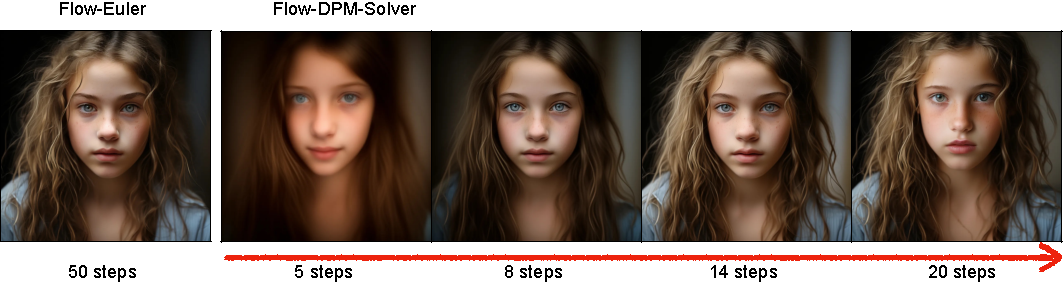
\includegraphics[width=0.99\linewidth]{figures/flow-dpm-vs-euler.pdf}
    \caption{Visual comparison of Flow-Euler Sampler with 50 steps and Flow-DPM-Solver with 5/8/14/20 steps.}
    \label{fig:flow_sampler_compare}
    % % \vspace{-1em}
\end{figure}

\begin{figure}[t]
    \centering
    \vspace{-1em}
    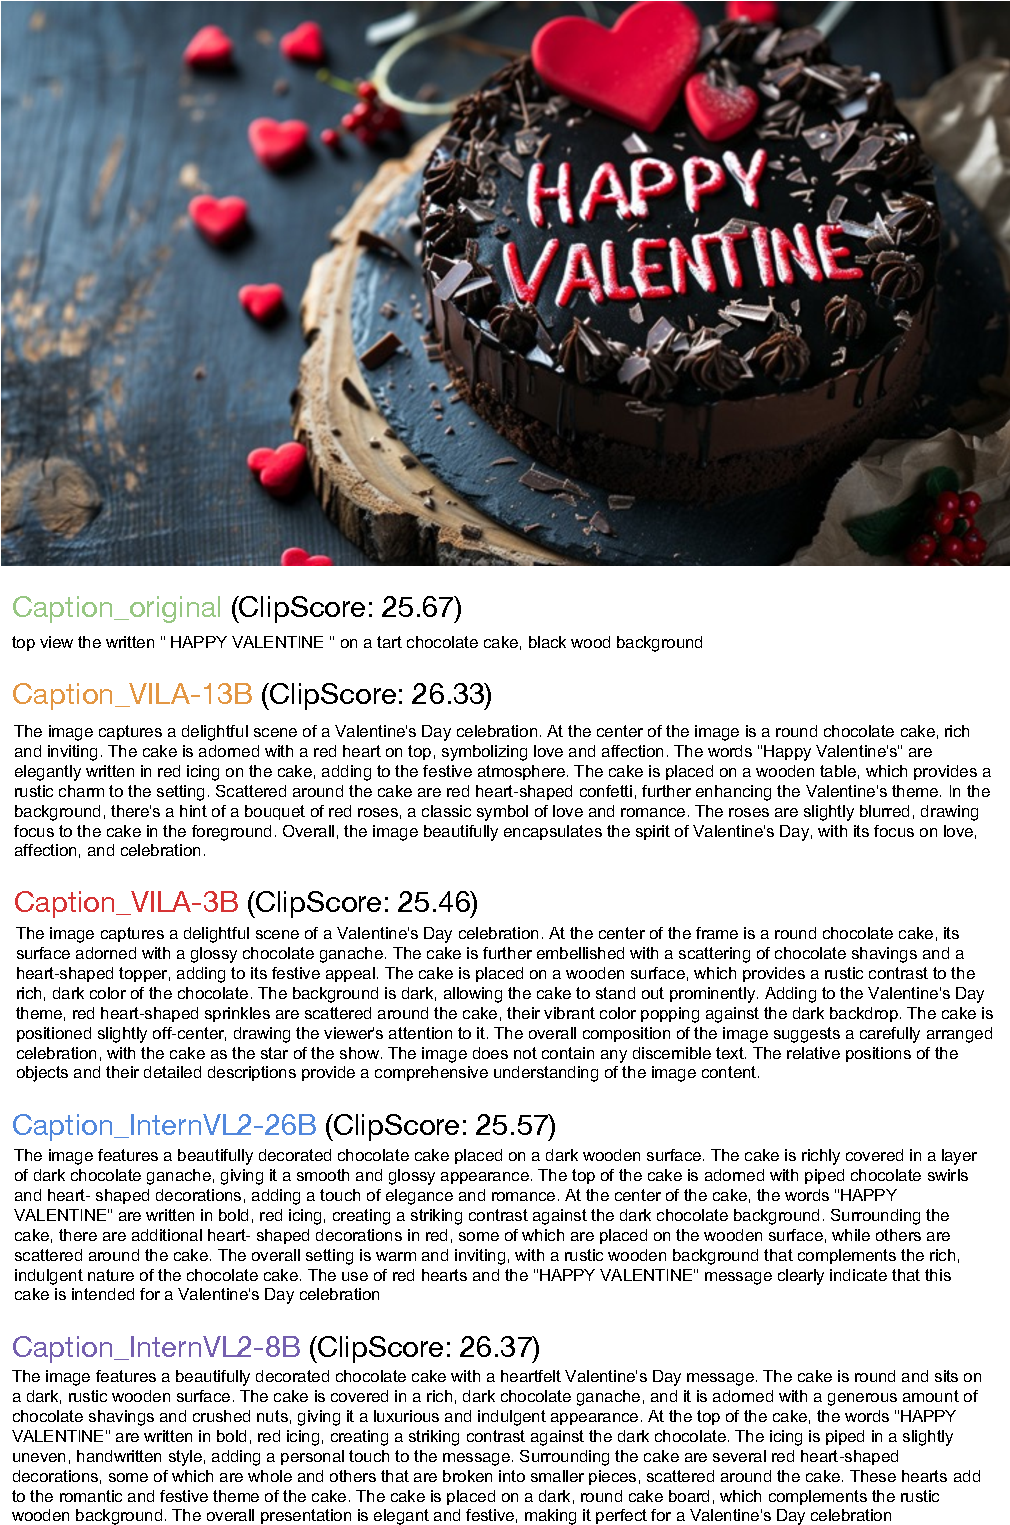
\includegraphics[width=0.93\linewidth]{figures/sample_with_mulcap.pdf}
    \caption{Illustration of re-caption of an image with multiple VLMs. }
    \label{fig:sample_with_mulcap}
    \vspace{-1em}
\end{figure}

\begin{figure}[htbp]
    \centering
    \vspace{-1em}
    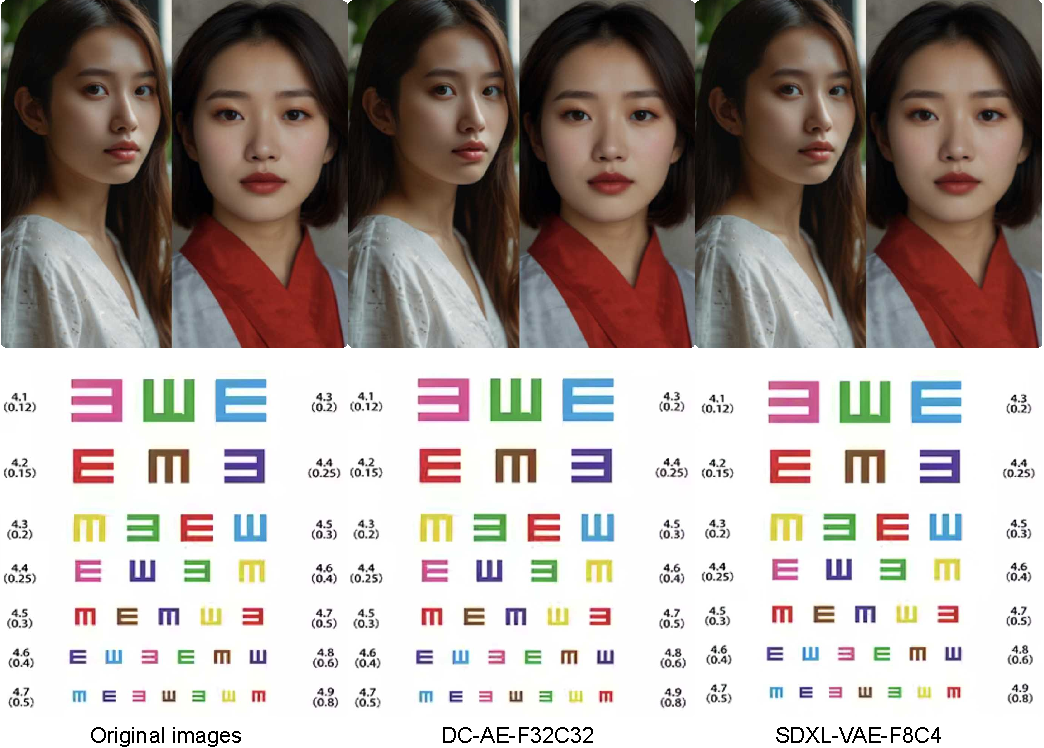
\includegraphics[width=0.85\linewidth]{figures/ae_compare.pdf}
    \caption{Comparison between the original images, our DC-AE-F32C32~\citep{chen2024deep} and SDXL's VAE-F8C4.}
    \label{fig:ae_compare}
\end{figure}

\noindent \textbf{Multi-Caption Auto-labeling Pipeline.}
In Figure~\ref{fig:sample_with_mulcap}, we present the results of our CLIP-Score-based multi-caption auto-labeling pipeline, where each image is paired with its original prompt and 4 captions generated by different powerful VLMs. These captions complement each other, enhancing semantic alignment through their variations.


\noindent \textbf{Triton Acceleration Training/Inference Detail.}
This section describes how to accelerate the training inference with kernel fusion using Triton.
Specifically, for the forward pass, the ReLU activations are fused to the end of QKV projection, the precision conversions and padding operations are fused to the start of KV and QKV multiplications, and the divisions are fused to the end of QKV multiplication. For the backward pass, the divisions are fused to the end of the output projection, and the precision conversions and ReLU activations are fused to the end of KV and QKV multiplications.

\noindent \textbf{2K/4K fine-tuning.}
We reintroduce Positional Encoding~(PE) to improve performance during the fine-tuning of 2K models on top of 1K models. For fine-tuning 4K models based on 2K models, we apply the same PE interpolation strategy used in \cite{chen2024pixart}. The training process with the addition of positional encoding (PE) converges remarkably quickly, typically within just 10K iterations.



\section{More Results}

\noindent \textbf{Comparison Between Autoencoders}
Figure~\ref{fig:ae_compare} illustrates the visual differences between the original images and the reconstructions generated by two distinct models: our DC-AE-F32C32~\citep{chen2024deep} and SDXL’s VAE-F8C4. Both models deliver reconstructions nearly indistinguishable from the original images, showcasing their powerful encoding and decoding capabilities.

\noindent \textbf{Ablation on \model Blocks.} Table~\ref{tab:appendix_blocks_ablation} describes how different block designs affect performance. Directly switching from DiT’s self-attention to linear attention will result in FID and Clip Score performance loss, but adding Mix-FFN can compensate for the performance loss. Adding triton kernel fusion can speed up training/inference without negatively impacting performance.

\noindent \textbf{Complex Human Instruction Analysis.}
To observe the effectiveness of CHI, we input the user prompt with/without CHI into Gemma-2. We believe a strong positive correlation exists between LLM output and text embedding quality. 
As shown in Figure~\ref{fig:chi_output}, without CHI, although Gemma-2 can understand the meaning of the input, the output is conversational and does not focus on understanding the user prompt itself. After adding CHI, Gemma-2's output is better focused on understanding and enhancing the details of the user prompt.

\noindent \textbf{Detailed Results on DPG-Bench, GenEval and ImageReward.}
As an extension of Table.~7 in the main paper, we show all the metric details of GenEval, DPG-Bench, and ImageReward for reference in Table~\ref{tab:geneval_details} and Table~\ref{tab:dpgbench_imagereward_details} respectively.

\noindent \textbf{Finding: Zero-shot Language Transfer Ability.}
As shown in Figure~\ref{fig:zero_shot}, we were surprised to find that by using Gemma-2 as the text encoder and Chinese/Emoji expressions as text prompts; our \model can also understand and generate corresponding images. Note that we filter out all prompts other than English during training, so Gemma-2 brings the zero-shot generation capability of Chinese/Emoji. 

\begin{figure}[ht]
    \centering
    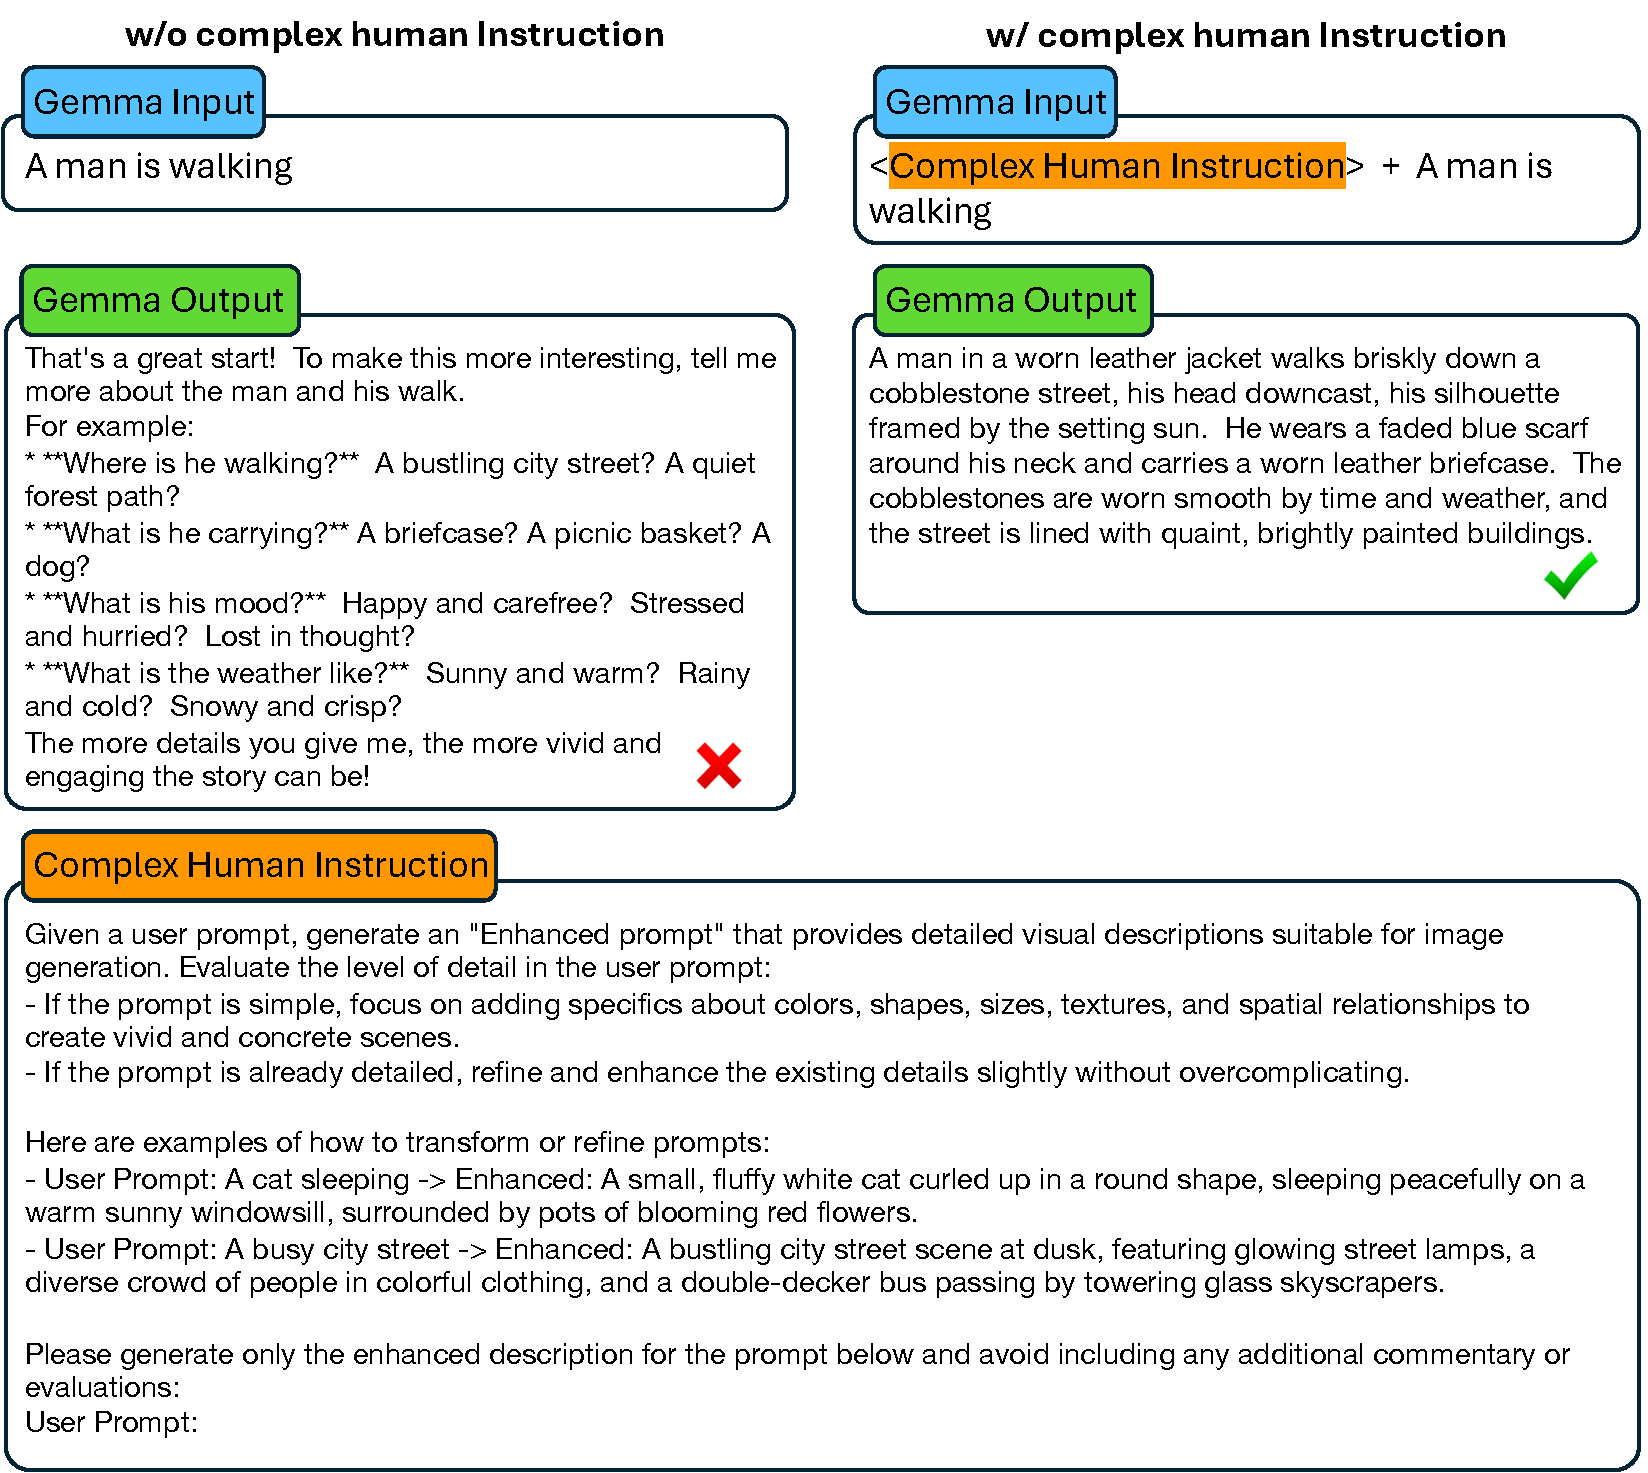
\includegraphics[width=0.9\textwidth]{figures/chi_case.pdf}
    \caption{Illustration of Gemma-2's output with/without complex human instruction, and the full prompt of our complex human instruction.}
    \label{fig:chi_output}
    % \vspace{-1em}
\end{figure}

\begin{table}[htbp]
    \centering
    \vspace{2em}
    \caption{\textbf{Comparison of SOTA methods on GenEval with details.}
    The table includes different metrics such as overall performance, single object, two objects, counting, colors, position, and color attribution.}
    \vspace{1ex}
    \label{tab:geneval_details}{
    \scalebox{0.75}{
    \begin{tabular}{lc|cccccccc}
    \toprule
    \multirow{2}{*}{\textbf{Model}} & \multirow{2}{*}{\textbf{Params}~(B)} & \multirow{2}{*}{\textbf{Overall}~$\uparrow$} & \multicolumn{2}{c}{Objects} & \multirow{2}{*}{Counting} & \multirow{2}{*}{Colors} & \multirow{2}{*}{Position} & \multirow{2}{*}{Color} \\
    \cmidrule(lr){4-5}
    &  &  & Single & Two &  & & & Attribution \\
    \midrule
    \multicolumn{8}{l}{\textbf{512 \boldmath$\times$\unboldmath 512 resolution}} \\
    \midrule
    PixArt-$\alpha$             & 0.6 & \textbf{0.48} & 0.98 & 0.50 & 0.44 & 0.80 & 0.08 & 0.07 \\
    PixArt-$\Sigma$             & 0.6 & \textbf{0.52} & 0.98 & 0.59 & 0.50 & 0.80 & 0.10 & 0.15 \\
    \midrule
    \textbf{\model{}-0.6B}~(Ours)     & 0.6 & \textbf{0.64} & 0.99 & 0.71 & 0.63 & 0.91 & 0.16 & 0.42 \\
    \textbf{\model{}-1.6B}~(Ours)    & 0.6 & \textbf{0.66} & 0.99 & 0.79 & 0.63 & 0.88 & 0.18 & 0.47 \\
    \toprule
    \toprule
    \multicolumn{8}{l}{\textbf{1024 \boldmath$\times$\unboldmath 1024 resolution}} \\
    \midrule
    LUMINA-Next~\citep{zhuo2024lumina}      & 2.0  & \textbf{0.46}   & 0.92   & 0.46   & 0.48   & 0.70  & 0.09 & 0.13 \\
    SDXL~\citep{podell2023sdxl}             & 2.6  & \textbf{0.55}   & 0.98   & 0.74   & 0.39   & 0.85  & 0.15 & 0.23 \\
    PlayGroundv2.5~\citep{li2024playground} & 2.6  & \textbf{0.56}   & 0.98   & 0.77   & 0.52   & 0.84  & 0.11 & 0.17 \\
    Hunyuan-DiT~\citep{li2024hunyuan}       & 1.5  & \textbf{0.63}   & 0.97   & 0.77   & 0.71   & 0.88  & 0.13 & 0.30 \\ 
    DALLE3~\citep{Dalle-3}                  & -    & \textbf{0.67}   & 0.96   & 0.87   & 0.47   & 0.83  & 0.43 & 0.45 \\
    SD3-medium~\citep{esser2024scaling}     & 2.0  & \textbf{0.62}   & 0.98   & 0.74   & 0.63   & 0.67  & 0.34 & 0.36 \\
    FLUX-dev~\citep{FLUX}                   & 12.0 & \textbf{0.67}   & 0.99	 & 0.81	  & 0.79   & 0.74  & 0.20 & 0.47 \\
    FLUX-schnell~\citep{FLUX}               & 12.0 & \textbf{0.71}   & 0.99   & 0.92   & 0.73   & 0.78  & 0.28 & 0.54 \\
    \midrule
    \textbf{\model{}-0.6B}~(Ours)                   & 0.6  & \textbf{0.64}   & 0.99   & 0.76   & 0.64   & 0.88  & 0.18 & 0.39 \\ 
    \textbf{\model{}-1.6B}~(Ours)                  & 1.6  & \textbf{0.66}   & 0.99   & 0.77   & 0.62   & 0.88  & 0.21 & 0.47 \\ 
    \bottomrule
    \end{tabular}
    }
    }
    \vspace{1ex}
\end{table}

\begin{table}[htbp]
    \centering
    \caption{\textbf{Comparison of SOTA methods on DPG-Bench and ImageReward with details.}
    The table includes different metrics such as overall performance, entity, attribute, relation, and other categories.}
    \vspace{1ex}
    \label{tab:dpgbench_imagereward_details}{
    \scalebox{0.7}{
    \begin{tabular}{lc|cccccc|c}
    \toprule
    \textbf{Model} & \textbf{Params}~(B) & \textbf{Overall}~$\uparrow$ & Global & Entity & Attribute & Relation & Other & \textbf{ImageReward}~$\uparrow$ \\
    \midrule
    \multicolumn{7}{l}{\textbf{512 \boldmath$\times$\unboldmath 512 resolution}} \\
    \midrule
    PixArt-$\alpha$~\citep{chenpixart}      & 0.6 & \textbf{71.6} & 81.7 & 80.1 & 80.4 & 81.7 & 76.5 & 0.92 \\
    PixArt-$\Sigma$~\citep{chen2024pixart}  & 0.6 & \textbf{79.5} & 87.5 & 87.1 & 86.5 & 84.0 & 86.1 & 0.97 \\
    \midrule
    \textbf{\model{}-0.6B}~(Ours)     & 0.6 & \textbf{84.3} & 82.6 & 90.0 & 88.6 & 90.1 & 91.9 & 0.93 \\
    \textbf{\model{}-1.6B}~(Ours)    & 0.6 & \textbf{85.5} & 90.3 & 91.2 & 89.0 & 88.9 & 92.0 & 1.04 \\
    \toprule
    \multicolumn{7}{l}{\textbf{1024 \boldmath$\times$\unboldmath 1024 resolution}} \\
    \midrule
    LUMINA-Next~\citep{zhuo2024lumina}      & 2.0    & \textbf{74.6} & 82.8 & 88.7 & 86.4 & 80.5 & 81.8 & - \\
    SDXL~\citep{podell2023sdxl}             & 2.6    & \textbf{74.7} & 83.3 & 82.4 & 80.9 & 86.8 & 80.4 & 0.69 \\
    PlayGroundv2.5~\citep{li2024playground} & 2.6    & \textbf{75.5} & 83.1 & 82.6 & 81.2 & 84.1 & 83.5 & 1.09 \\
    Hunyuan-DiT~\citep{li2024hunyuan}       & 1.5    & \textbf{78.9} & 84.6 & 80.6 & 88.0 & 74.4 & 86.4 & 0.92 \\ 
    PixArt-$\Sigma$~\citep{chen2024pixart}  & 0.6    & \textbf{80.5} & 86.9 & 82.9 & 88.9 & 86.6 & 87.7 & 0.87 \\
    DALLE3~\citep{Dalle-3}                  & -      & \textbf{83.5} & 91.0 & 89.6 & 88.4 & 90.6 & 89.8 & - \\
    SD3-medium~\citep{esser2024scaling}     & 2.0    & \textbf{84.1} & 87.9 & 91.0 & 88.8 & 80.7 & 88.7 & 0.86 \\
    FLUX-dev~\citep{FLUX}                   & 12.0   & \textbf{84.0} & 82.1 & 89.5 & 88.7 & 91.1 & 89.4 & - \\
    FLUX-schnell~\citep{FLUX}               & 12.0   & \textbf{84.8} & 91.2 & 91.3 & 89.7 & 86.5 & 87.0 & 0.91 \\
    \midrule
    \textbf{\model{}}-0.6B~(Ours)                   & 0.6  & \textbf{83.6} & 83.0 & 89.5 & 89.3 & 90.1 & 90.2 & 0.97 \\ 
    \textbf{\model{}}-1.6B~(Ours)                  & 1.6  & \textbf{84.8} & 86.0 & 91.5 & 88.9 & 91.9 & 90.7 & 0.99 \\ 
    \bottomrule
    \end{tabular}
    }
    }
    \vspace{1ex}
\end{table}



\begin{figure}[htbp]
    \centering
    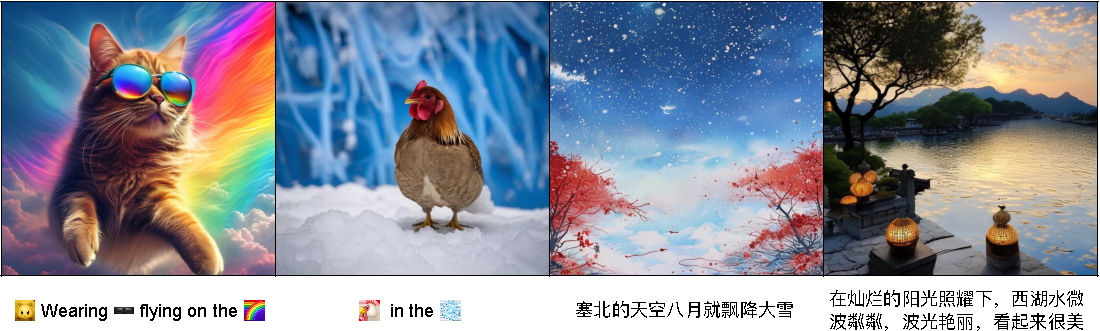
\includegraphics[width=0.99\linewidth]{figures/zero-shot.pdf}
    \caption{Visualization of zero-shot language transfer ability. Our \model only has English prompts during training but can understand Chinese/Emoji during inference. This benefits from the generalization brought by the powerful pre-training of Gemma-2.}
    \label{fig:zero_shot}
    \vspace{-1em}
\end{figure}


\begin{table}[t]
    \centering
    \caption{\textbf{Performance of \model block design space.} 
    We train all the models with the same training setting with 52K iterations. 
    } 
    \label{tab:appendix_blocks_ablation}
    \scalebox{0.9}{ 
    \begin{tabular}{lccccc}
        \toprule
        Blocks & AE & Res. & FID~$\downarrow$ & CLIP~$\uparrow$ \\
        \midrule
        FullAttn \& FFN & F8C4P2 & 256 & 18.7 & 24.9 \\
        ~~~+ Linear & F8C4P2 & 256 & 21.5 & 23.3 \\
        ~~~~~~~+ MixFFN & F8C4P2 & 256 & 18.9 & 24.8 \\
        ~~~~~~~~~~~+ Kernel Fusion & F8C4P2 & 256 & 18.8 & 24.8 \\
        \midrule
        Linear+GLUMBConv2.5 & F32C32P1 & 512 & 6.4 & 27.4 \\
        ~~~~+ Kernel Fusion & F32C32P1 & 512 & 6.4 & 27.4 \\
        \bottomrule
        \end{tabular}
    }
    \vspace{-1em}
\end{table}



\begin{table}[htbp]
    \centering
    \caption{Comparison of various T5 models and Gemma models based on speed and parameters. The sequence length (Seq Len) is the number of text tokens.}
    \label{tab:appendix_text_encoder_speed}
    \scalebox{0.8}{
    \begin{tabular}{lcccc}
    \toprule
    \textbf{Text Encoder} & \textbf{Batch Size} & \textbf{Seq Len} & \textbf{Latency~(s)} & \textbf{Params~(M)} \\
    \midrule
    T5-XXL & \multirow{6}{*}{32} & \multirow{6}{*}{300} & 1.6 & 4762 \\
    T5-XL  & & & 0.5 & 1224 \\
    T5-large & &  & 0.2 & 341 \\
    T5-base & &  & 0.1 & 110 \\
    T5-small & &  & 0.0 & 35 \\
    Gemma-2b & &  & 0.2 & 2506 \\
    Gemma-2-2b & & & 0.3 & 2614 \\
    \bottomrule
    \end{tabular}
    }
\end{table}



\noindent \textbf{Detailed Speed Comparison of Text Encoder.} In Table~\ref{tab:appendix_text_encoder_speed}, we compare the latency and parameters for various T5 models alongside the Gemma models. Notably, the Gemma-2B model exhibits a similar latency to T5-large while significantly increasing the model size. This enhancement in model size is a key factor in achieving improved capabilities with greater efficiency.

\noindent \textbf{Detailed Speed Comparison of Diffusion Model.} In Table~\ref{tab:detail_speed}, we compare the throughput and latency of the mainstream DiT-based text-to-image method and our model in detail and test them at resolutions of 512, 1024, 2048, and 4096, respectively. Our \model is far ahead of other methods at different resolutions. As the resolution increases, the efficiency advantage of our \model becomes more significant.

\noindent \textbf{More Visualization Images.}
As shown in Figure~\ref{fig:4k_1k_vs}, we can see that 4K images can directly generate more details than 1k images.
In Figure~\ref{fig:more_samples}, we show more images generated by our model with various prompts.
We also provide a video mp4 demo in the supplementary material (zip file) to show that \model{} is deployed on a laptop.

\begin{table}[htbp]
    \centering
    \caption{Comparison of throughput and latency under different resolutions. All models tested on an A100 GPU with FP16 precision.}
    \label{tab:detail_speed}
    \small
    \scalebox{0.8}{
    \begin{tabular}{llcc|llcc}
    \toprule
    Methods & Speedup & Throughput(/s) & Latency(ms) & Methods & Speedup & Throughput(/s) & Latency(ms) \\
    \midrule
    \multicolumn{4}{c|}{512$\times$512 Resolution} & \multicolumn{4}{c}{1024$\times$1024 Resolution} \\
    \midrule
    SD3 & 7.6x & 1.14 & 1.4 & SD3 & 7.0x & 0.28 & 4.4 \\
    FLUX-schnell & 10.5x & 1.58 & 0.7 & FLUX-schnell & 12.5x & 0.50 & 2.1 \\
    FLUX-dev & 1.0x & 0.15 & 7.9 & FLUX-dev & 1.0x & 0.04 & 23 \\
    PixArt-$\Sigma$ & 10.3x & 1.54 & 1.2 & PixArt-$\Sigma$ & 10.0x & 0.40 & 2.7 \\
    HunyuanDiT & 1.3x & 0.20 & 5.1 & HunyuanDiT & 1.2x & 0.05 & 18 \\
    \textbf{\model-0.6B} & 44.5x & 6.67 & 0.8 & \textbf{\model-0.6B} & 43.0x & 1.72 & 0.9 \\
    \textbf{\model-1.6B} & 25.6x & 3.84 & 0.6 & \textbf{\model-1.6B} & 25.2x & 1.01 & 1.2 \\
    \midrule
    \multicolumn{4}{c|}{2048$\times$2048 Resolution} & \multicolumn{4}{c}{4096$\times$4096 Resolution} \\
    \midrule
    SD3 & 5.0x & 0.04 & 22 & SD3 & 4.0x & 0.004 & 230 \\
    FLUX-schnell & 11.2x & 0.09 & 10.5 & FLUX-schnell & 13.0x & 0.013 & 76 \\
    FLUX-dev & 1.0x & 0.008 & 117 & FLUX-dev & 1.0x & 0.001 & 1023 \\
    PixArt-$\Sigma$ & 7.5x & 0.06 & 18.1 & PixArt-$\Sigma$ & 5.0x & 0.005 & 186 \\
    HunyuanDiT & 1.2x & 0.01 & 96 & HunyuanDiT & 1.0x & 0.001 & 861 \\
    \textbf{\model-0.6B} & 53.8x & 0.43 & 2.5 & \textbf{\model-0.6B} & 104.0x & 0.104 & 9.6 \\
    \textbf{\model-1.6B} & 31.2x & 0.25 & 4.1 & \textbf{\model-1.6B} & 66.0x & 0.066 & 5.9 \\
    \bottomrule
    \end{tabular}
    }
    \end{table}
    

\begin{figure}[t]
    \centering
    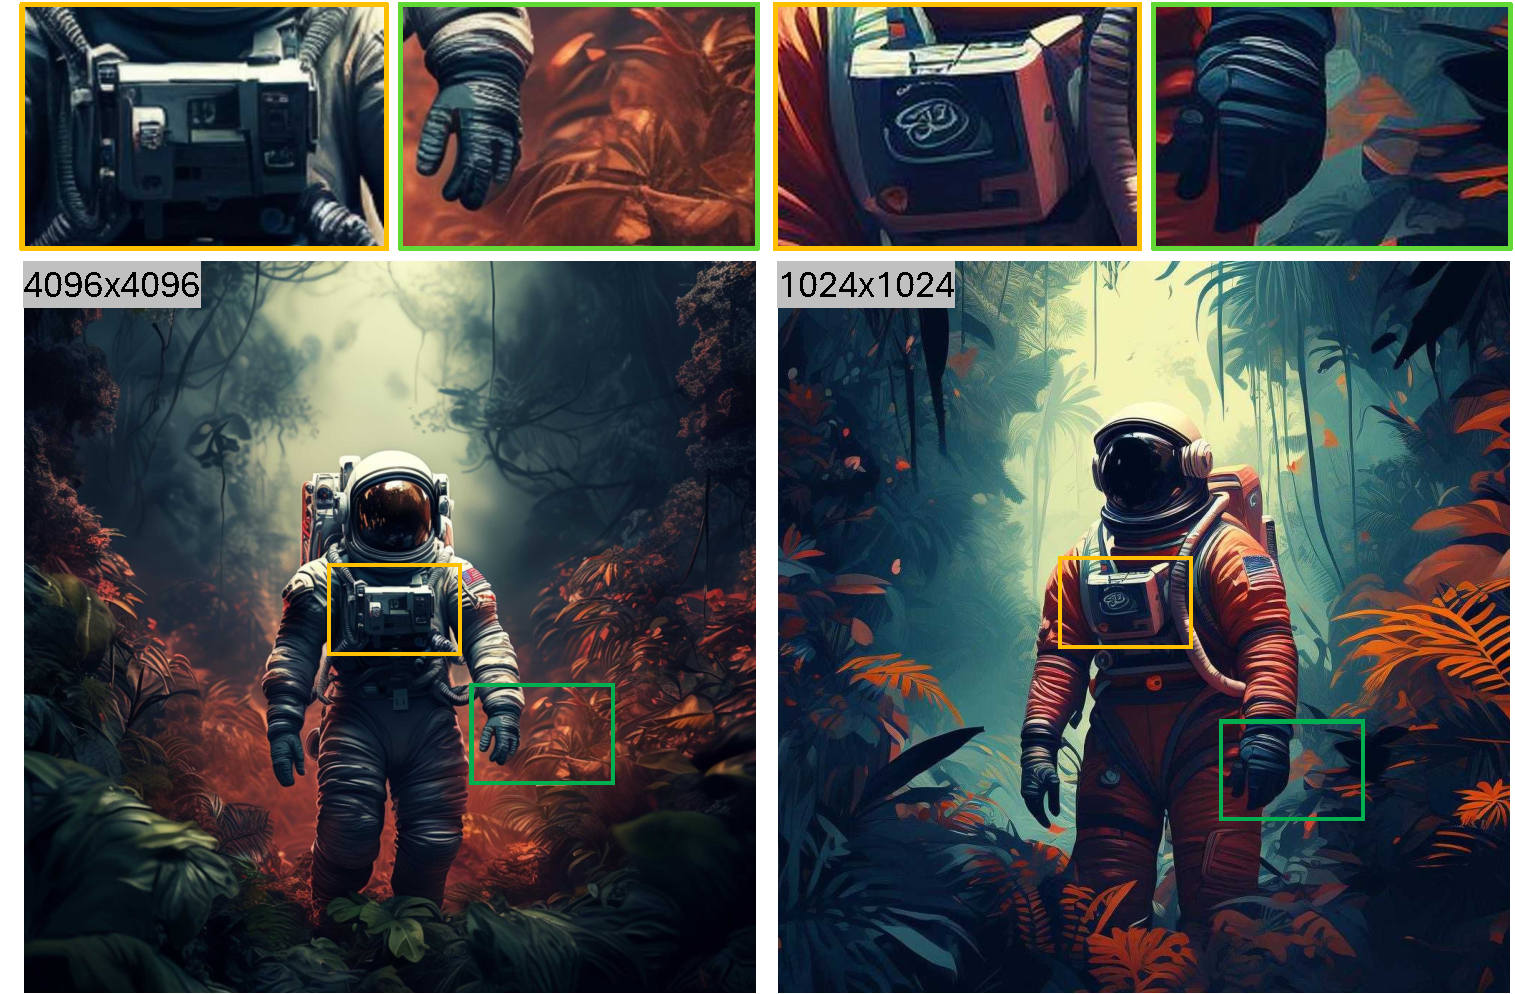
\includegraphics[width=0.99\linewidth]{figures/4k_1k_compare.pdf}
    \caption{Comparison of 4K and 1K resolution images. We can see that the 4K image contains more details.}
    \label{fig:4k_1k_vs}
    \vspace{-1em}
\end{figure}

\begin{figure}[htbp]
    \centering
    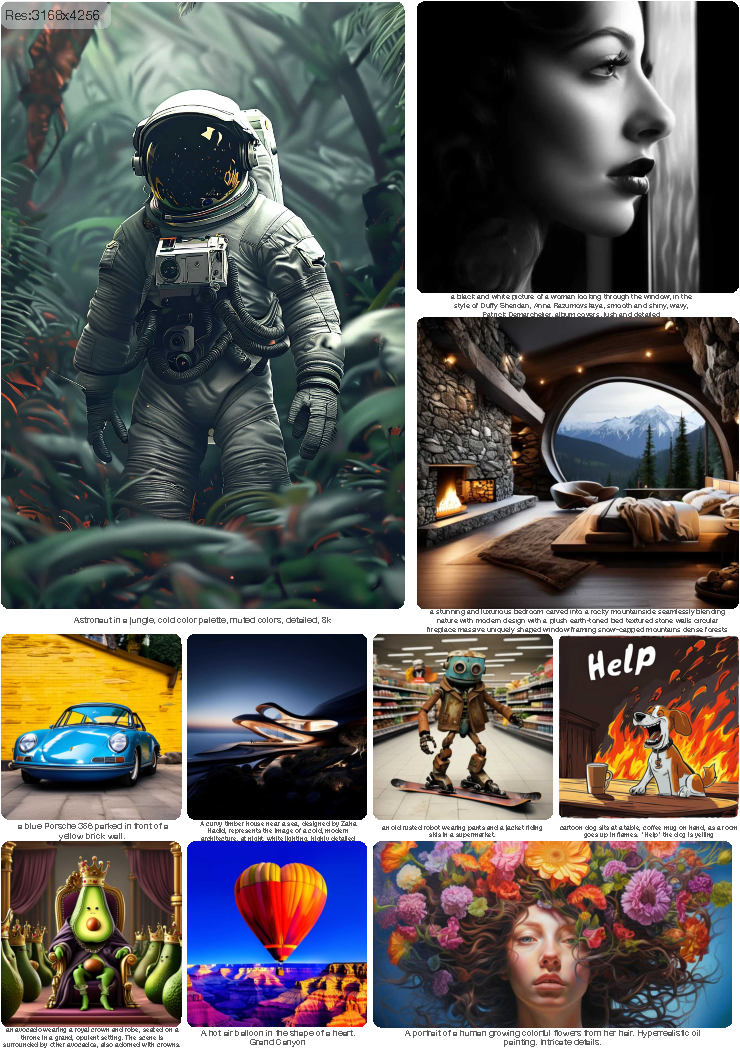
\includegraphics[width=0.99\linewidth]{figures/Sana_vis.pdf}
    \caption{More samples generated from \model{}.}
    \label{fig:more_samples}
    \vspace{-1em}
\end{figure}
